\documentclass[openright,letterpaper,12pt]{book}
\usepackage[utf8]{inputenc}
\usepackage[french]{babel}
\usepackage{graphicx}
\usepackage{float}
\usepackage{pdfpages}
\usepackage[plainheadsepline,markcase=ignoreuppercase]{scrlayer-scrpage}
\usepackage{titlesec}
\usepackage{tocloft}
\usepackage{hyperref}
\usepackage{geometry}
\usepackage{listings}
\usepackage[dvipsnames]{xcolor}
\hypersetup{
		pdfauthor={Alexandre Dumont},
		pdftitle={MegaYoko},
		pdfsubject={Guide d'utilisateur},
		pdfkeywords={Manuel},
		%pdftex,
		colorlinks=true,
		breaklinks=true,
		urlcolor=RoyalBlue,
		linkcolor=RoyalBlue,
		citecolor=RoyalBlue,
		bookmarksopen=true,
		unicode=true
}
\usepackage{bookmark}
\usepackage{cmap} % Doit
\usepackage[T1]{fontenc}
\usepackage[hyperpageref]{backref}

\geometry{letterpaper, inner=1.5in, outer=1.0in, tmargin=1.5in, bmargin=1.0in, twoside=false}

\pagestyle{scrheadings}
%\renewcommand{\chaptermark}[1]{\markboth{{\thechapter. #1}}{}}
%\renewcommand{\sectionmark}[1]{aa}
\setlength{\headheight}{18pt}
\setlength{\footheight}{18pt}

\definecolor{codegreen}{rgb}{0,0.6,0}
\definecolor{codegray}{rgb}{0.5,0.5,0.5}
\definecolor{codepurple}{rgb}{0.58,0,0.82}
\definecolor{backcolour}{rgb}{1,1,1}

\lstdefinestyle{mystyle}{
	emph={get, output\_en, level},
    backgroundcolor=\color{backcolour},   
    commentstyle=\color{codegreen},
    keywordstyle=\color{codegreen},
    emphstyle=\color{codegreen},
    numberstyle=\tiny\color{codegray},
    stringstyle=\color{codepurple},
    basicstyle=\ttfamily\normalsize,
    breakatwhitespace=false,         
    breaklines=true,                 
    captionpos=b,                    
    keepspaces=true,                 
    numbers=left,                    
    numbersep=5pt,                  
    showspaces=false,                
    showstringspaces=false,
    showtabs=false,                  
    tabsize=2,
	aboveskip=20pt,
	belowskip=20pt,
}

\lstset{style=mystyle}

\begin{document}
\pagenumbering{gobble}
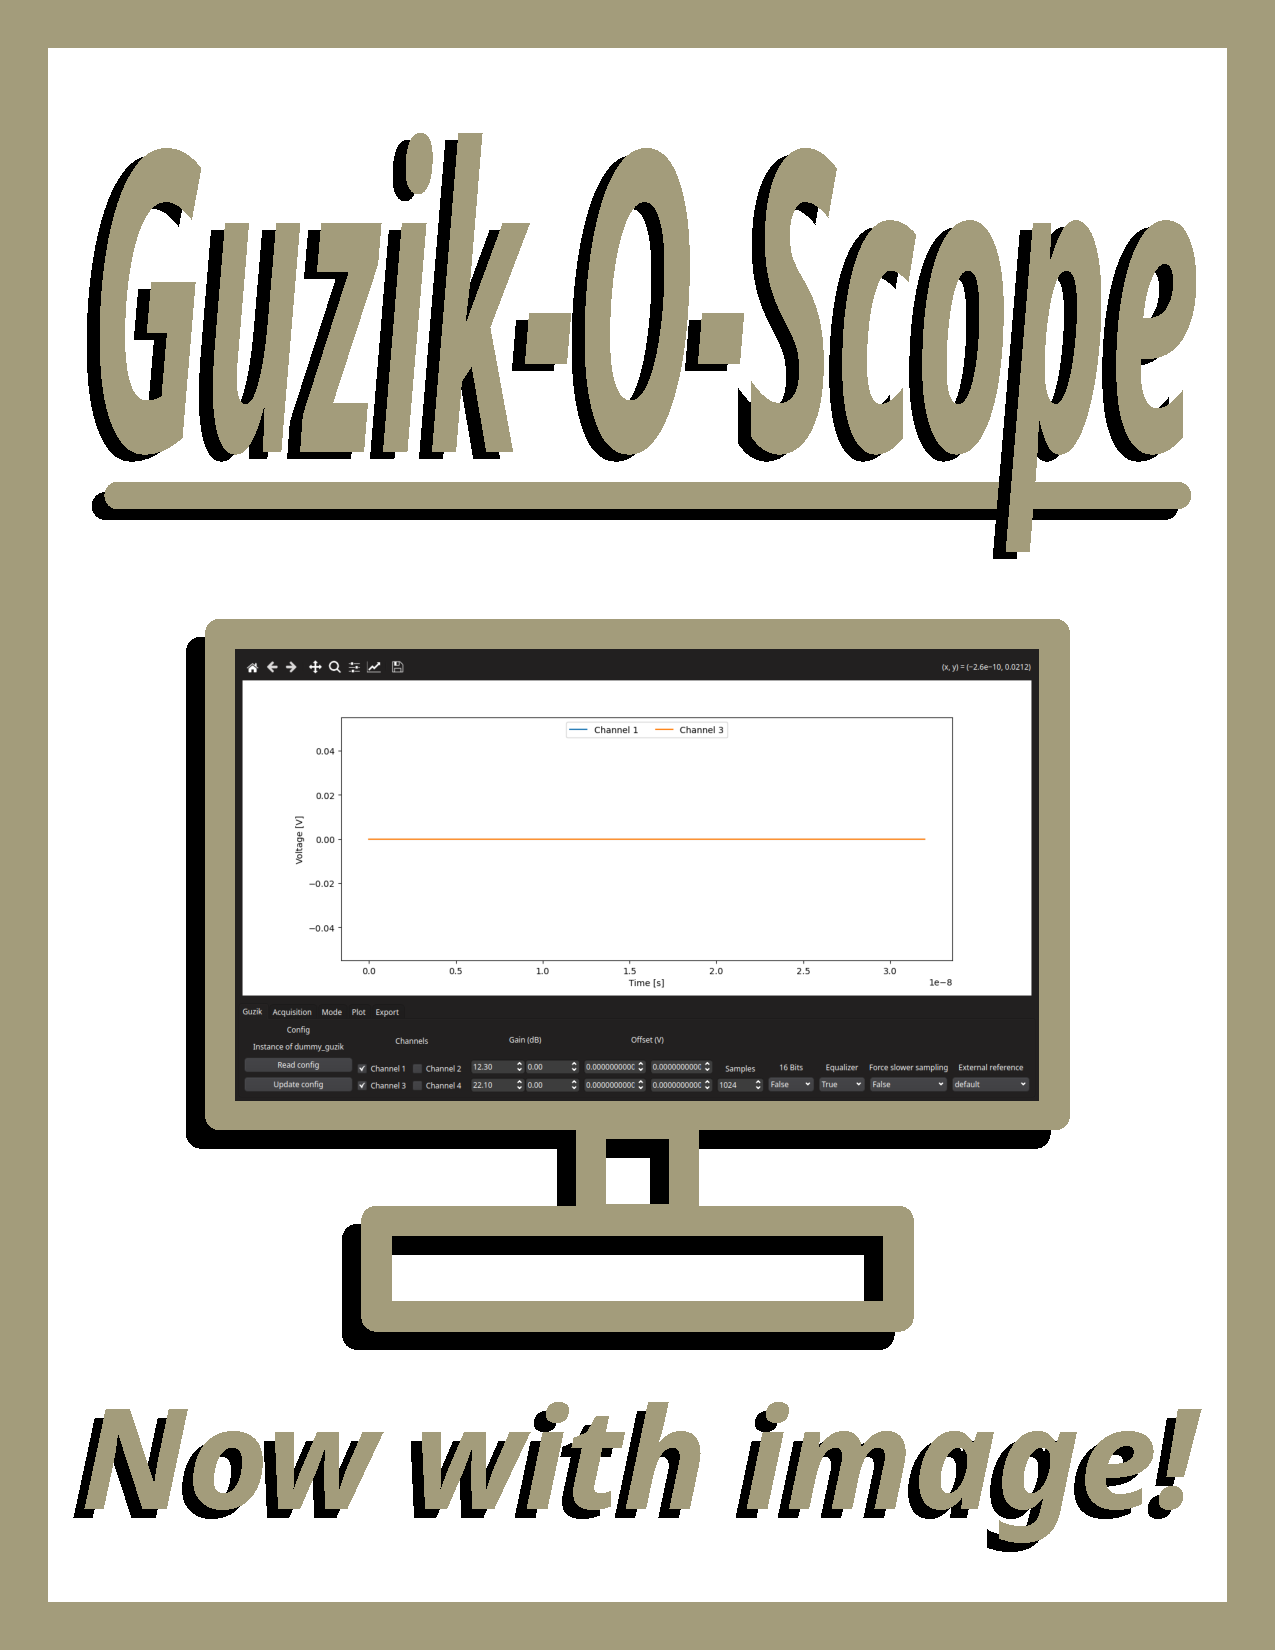
\includepdf[noautoscale=true, scale=1]{Figures/Pagetitre/pagetitre.pdf}
\clearpage\null\thispagestyle{empty}\clearpage
\thispagestyle{empty}
{\ } 

\vspace{3cm}
\noindent
{\fontsize{35.83pt}{40pt}\selectfont\bf Guzik-O-Scope\\} 
{\Large\bf Guide de l'utilisateur}

\vspace{10cm}\noindent
{\huge\bf Alexandre Dumont}\\
{\large ReuletLab}

\clearpage\null\thispagestyle{empty}

\renewcommand{\tableofcontents}
             {
                \clearpage
                \chapter*{\pdfbookmark[chapter]{\contentsname}{toc}
                          \contentsname}
                \csname @starttoc\endcsname{toc}
             }
\frontmatter
\chapter*{Garantie}
\addcontentsline{toc}{chapter}{Garantie}
Les instructions, le code et ce manuel sont fournis sans garanties et sans 
support et peuvent ne pas fonctionner.
\clearpage\null\thispagestyle{empty}

\tableofcontents
\clearpage\null\thispagestyle{empty}

\mainmatter

\clearpage
\chapter*{Installation}
\addcontentsline{toc}{chapter}{Installation}
Ce chapitre explique la procédure pour installer le code Python pour le 
Guzik-O-Scope. 
L'installation est facultative. 
Pour utiliser le code sans l'installer, il faut tout de même le télécharger et 
s'assurer que le code soit dans un répertoire accessible par l'instance de 
Python.

\section*{Obtenir les dépendances}
Pour pouvoir fonctionner, le Guzik-O-Scope à plusieurs dépendances, dont numpy 
et matplotlib, qui peuvent être facilement installée, si elles ne le sont pas 
déjà, et la librairie \verb+SignalProcessing+. 
Celle dernière est une librairie maison qui se trouve sur Github à l'adresse 
\href{https://github.com/a-dumont/SignalProcessing}
{https://github.com/a-dumont/SignalProcessing}. 
Pour installer cette libraire, il est nécessaire de compiler du code, soit à 
partir de cygwin sur Windows, où directement avec \verb+gcc+ sur Linux.

\subsection*{Windows}
Pour que le code puisse compiler correctement, certaines dépendances doivent 
êtres installées à partir de cygwin, notamment, \verb+CMake+, \verb+MinGW+, 
\verb+FFTW3+ et \verb+Pybind11+. 
Une fois ces dépendances installées via l'installateur de cygwin, il faut 
ouvrir
exécuter les commandes suivantes.
\begin{lstlisting}[language=Bash]
git clone https://github.com/a-dumont/SignalProcessing
cd SignalProcessing/
mkdir build && cd build
CXX=/usr/bin/x86_64-w64-mingw32-g++.exe cmake .. 
cmake --build . && cmake --install .
cd .. && /c/Anaconda3/python.exe setup.py install
\end{lstlisting}
Il est très important qu'a la dernière ligne, la commande \verb+python.exe+ 
soit celle du système et que son emplacement peut être différent de l'exemple 
fourni ici.
Puisqu'il faut installer les dépendances, les privilèges d'administrateur 
peuvent êtres requis. 
Si c'est le cas, le terminal cygwin doit être ouvert en tant qu'administrateur.

\subsection*{Linux}
Pour que le code puisse compiler correctement, certaines dépendances doivent 
êtres installées donc, \verb+CMake+, \verb+FFTW3+ et \verb+Pybind11+. 
Une fois ces dépendances installées, il faut 
exécuter les commandes suivantes.
\begin{lstlisting}[language=Bash]
git clone https://github.com/a-dumont/SignalProcessing
cd SignalProcessing/
mkdir build && cd build
cmake .. && cmake --build . && cmake --install .
cd .. && python setup.py install
\end{lstlisting}
Puisqu'il faut installer les dépendances, les privilèges d'administrateur 
peuvent êtres requis. 

\section*{Obtenir le code}
La façon la plus simple d'obtenir le code est d'utiliser \verb+git+ à partir 
d'un terminal, que ce soit sur Windows, macOS où Linux. 
Plus spécifiquement, il faut naviguer au répertoire choisi via le terminal et 
exécuter la commande suivante,

\begin{lstlisting}[language=Bash]
git clone https://github.com/a-dumont/GuzikGUI
\end{lstlisting}

Une façon alternative d'obtenir le code source est d'accéder au dépôt sur 
Github via un navigateur web et de télécharger le code dans une archive de 
type ZIP. 
Une fois cette archive décompresser dans le répertoire voulu, l'installation 
peut procéder normalement.

\section*{Installation}
Pour installer le code du Guzik-O-Scope comme un module Python, il faut 
naviguer dans le répertoire \verb+GuzikGUI+ à partir d'un terminal et lancer 
la commande,
\begin{lstlisting}[language=Bash]
python setup.py install
\end{lstlisting}
Il est possible que l'installation requiert les privilèges d'administrateur. 

\chapter*{Utilisation}
\addcontentsline{toc}{chapter}{Utilisation}
Le Guzik-O-Scope est fait pour fonctionner avec pyHegel et son implémentation 
du Guzik. 
Par contre, le code contient une classe permettant d'imiter le comportement du 
Guzik qui est instanciée automatiquement si le code ne parvient pas à 
charger l'implémentation de pyHegel. 
Ce cas est particulièrement pratique pour tester des modifications au code du 
Guzik-O-Scope sans avoir besoin du matériel physique.
\section*{Application seule}
Pour lancer le Guzik-O-Scope il suffit d'exécuter la commande suivante à partir 
d'un terminal.
\begin{lstlisting}[language=Bash]
python -m GuzikGUI
\end{lstlisting}
Il est possible d'écrire un script qui contient cette commande et de créer un 
raccourci pour celui-ci pour lancer l'application en un clic.

\section*{Application avec debug}
Pour une raison ou une autre, il peut être utile d'avoir accès aux variables 
qu'utilise le Guzik-O-Scope. 
Il est possible de lancer l'application via \verb+Ipython+ de manière 
interactive avec les commandes suivantes.
\begin{lstlisting}[language=Python]
from GuzikGUI import launch
application, window = launch()
\end{lstlisting}
L'objet \verb+window+ contient toute les variables intéressantes.
\clearpage\null\thispagestyle{empty}

\chapter*{Fonctionnalités}
\addcontentsline{toc}{chapter}{Fonctionnalités}
L'interface du Guzik-O-Scope est séparée en plusieurs onglets, ce chapitre 
passera, rapidement, en revue le rôle de chacun de ces onglets.

\section*{Guzik}
\begin{center}
		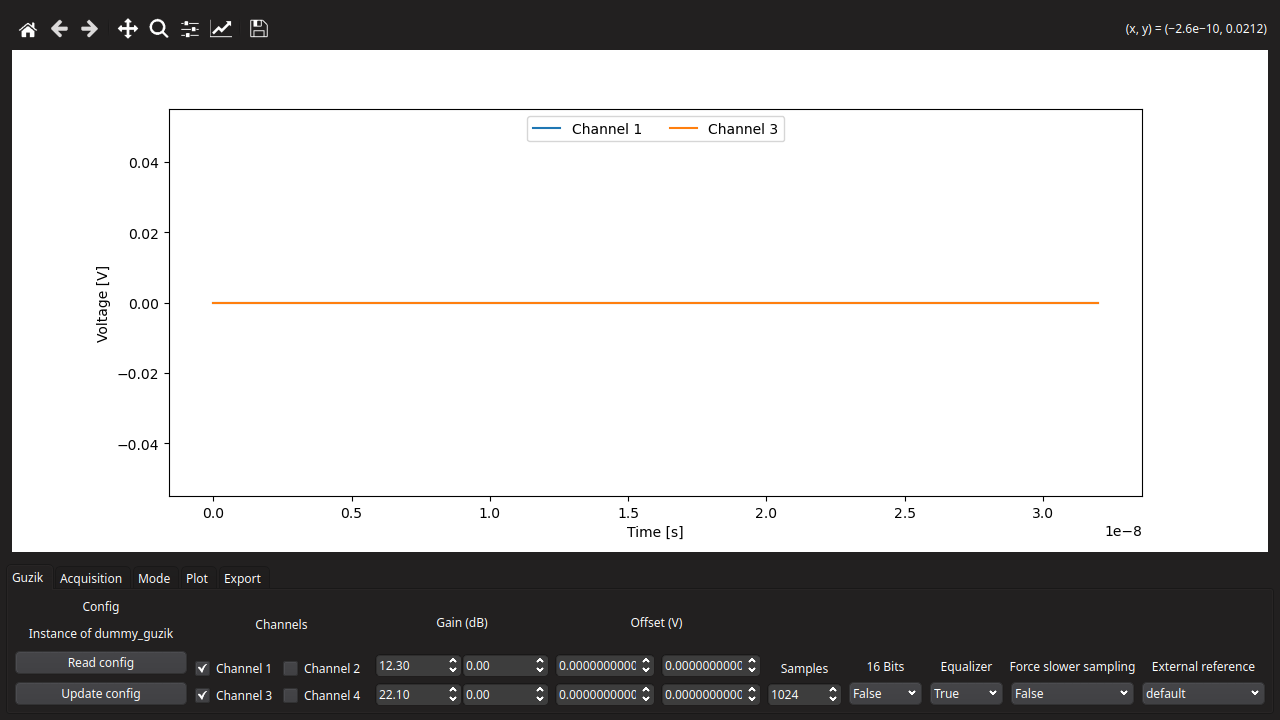
\includegraphics[width=\textwidth]{Figures/Guzik.png}
\end{center}

Ce premier onglet sert à configurer les différents paramètres du Guzik. 
Il est possible d'y changer les canaux utiliser pour la détection, le gain et 
le décalage en tension sur chacun des canaux. 
Les paramètre restants sont le nombre de points pour chaque mesure, la 
résolution de chaque point de mesure, l'égaliseur, la fréquence de mesure et 
la présence d'un signal de référence externe. 
Pour envoyer les modifications effectuées à l'instrument, il faut cliquer sur 
le bouton \textit{Update config}. 
Pour lire la configuration actuelle de l'instrument, il faut cliquer sur le 
bouton \textit{read config}.

\section*{Acquisition}\vspace{1cm}

L'onglet \textit{Acquisition} permet de choisir si les mesures seront moyennées 
ou non, et si oui combien de fois. 
Pour activer le moyennage, sous \textit{Averaging} choisir l'option 
\textit{True} et entrer un nombre dans le champ de texte.
Il est aussi possible de choisir entre des mesures individuelle ou en continu 
en utilisant les boutons \textit{Single} et \textit{Continuous} respectivement. 
Pour une mesure individuelle, le Guzik-O-Scope moyenne le nombre de mesures 
spécifié et affiche le résultat en temps réel. 
Pour des mesures en continu, la moyenne est cyclique, c'est-à-dire que qu'à 
chaque fois que le nombre de mesures spécifié est atteint, la moyenne se 
réinitialise.\vspace{1cm}

\begin{center}
		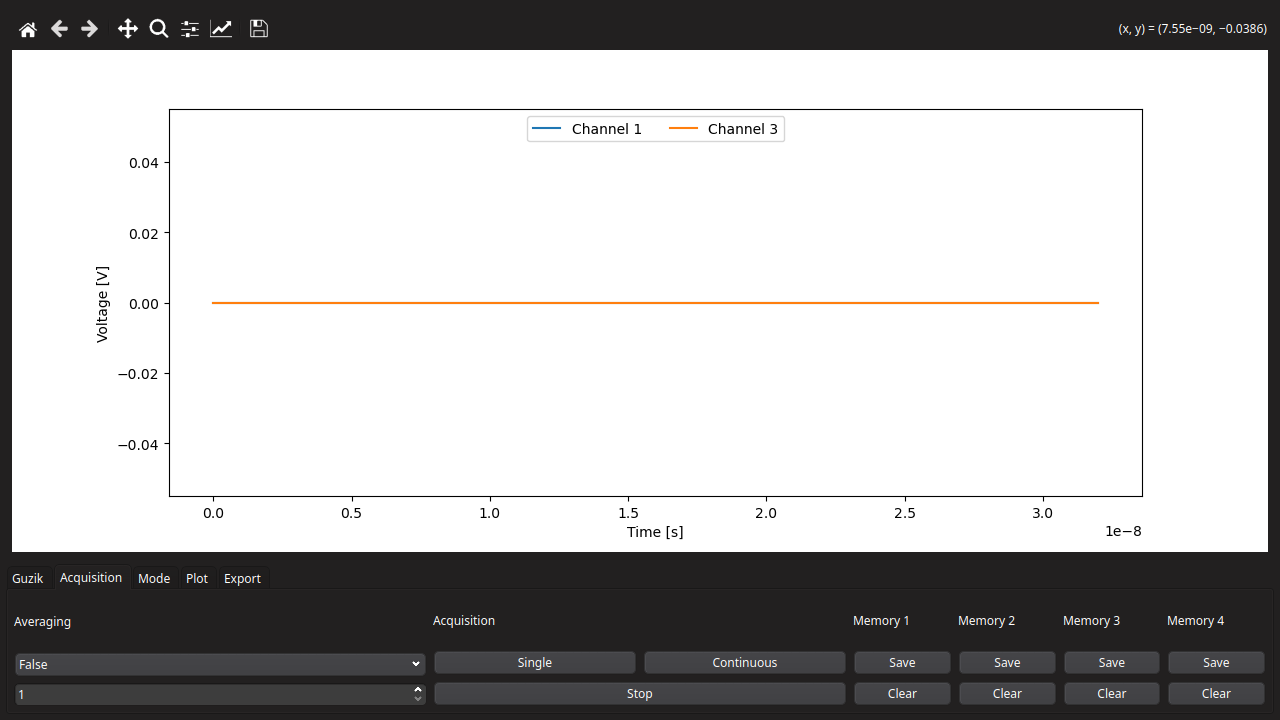
\includegraphics[width=\textwidth]{Figures/Acquisition.png}
\end{center}\vspace{1cm}

Comme le Guzik-O-Scope n'implémente pas de parallélisation, lorsque des mesures 
sont en cours l'interface graphique répond plus lentement. 
Pour retrouver le contrôle complet de l'interface il est possible d'interrompre 
une mesure en continue ou le moyennage d'une mesure individuelle en utilisant 
le bouton \textit{stop}.
Finalement, cet onglet permet aussi de stocker jusqu'à quatre courbes en 
mémoire pour permettre la comparaison entre différentes mesures en utilisant 
les différents boutons \textit{save} et \textit{clear}.\clearpage

\section*{Mode}\vspace{1cm}

L'onglet \textit{Mode} permet de choisr le type de mesure qui sera effectué par 
le Guzik-O-Scope. 
Il est possible de changer entre des mesures temporelles et des mesures en 
fréquence en changeant la valeur du champ \textit{Domain}. 
Pour l'espace du temps ou l'espace des fréquences les différentes mesures 
disponibles sont listées dans le champ \textit{Mode} juste en dessous de 
\textit{Domain}. 
En temps, les mesures disponibles sont, \textit{1D~Histogram} qui trace les 
histogrammes en une dimension sur chaque canal de mesure actif, 
\textit{2D Histogram} qui trace l'histogramme en deux dimensions des deux 
canaux actifs et finalement \textit{Time series} qui trace le signal brut de 
chaque canal.\vspace{1cm}

\begin{center}
		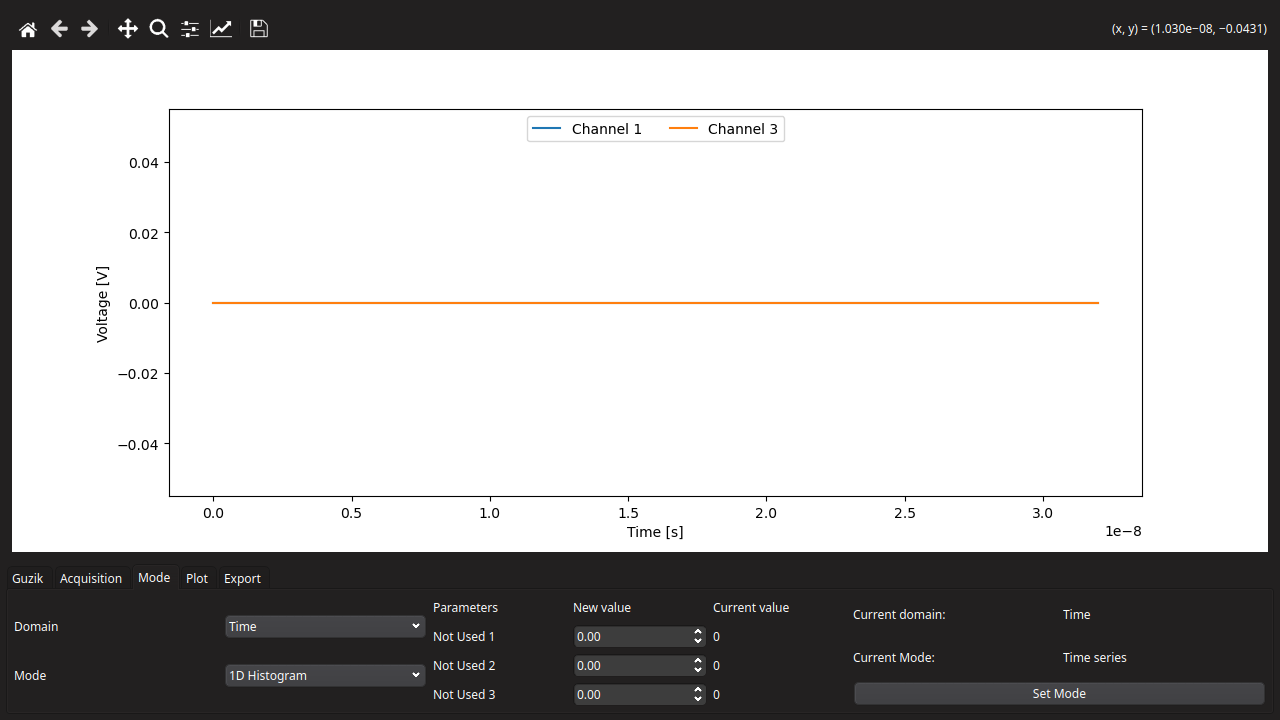
\includegraphics[width=\textwidth]{Figures/Mode.png}
\end{center}\vspace{1cm}

En fréquence, les mesures disponibles sont \textit{Power Spectrum} qui trace 
la densité spectrale de bruit sur chaque canal actif et \textit{Cross Power 
Spectrum} qui trace le module de la corrélation croisée entre les deux canaux 
actifs. 
Ces deux fonctions utilise le paramètre \textit{Block Size} qui permet de 
choisir la taille des blocs utilisés pour les transformés de Fourier. 
Pour changer le type de mesure ou un des paramètres comme \textit{Block Size}, 
il est nécessaire de cliquer le bouton \textit{Set Mode}.\clearpage

\section*{Plot}\vspace{1cm}

Présentement, l'onglet \textit{Plot} est peu utile mais le but est qu'il serve 
à changer le type de graphique pour une mesure donnée.
%\begin{center}
%		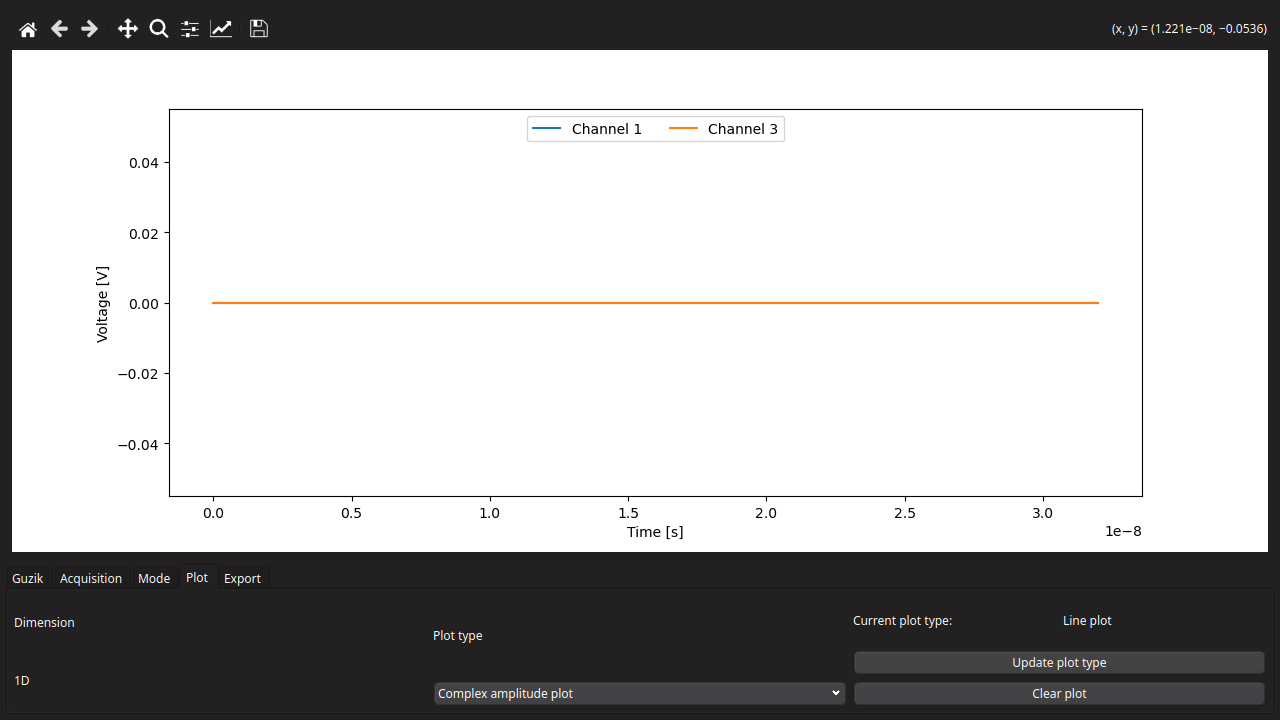
\includegraphics[width=\textwidth]{Figures/Plot.png}
%\end{center}

\section*{Export}\vspace{1cm}

Le dernier onglet, \textit{Export}, permet d'exporter les données vers un 
fichier. 
Il est possible de sauvegarder les données de la dernière mesure ainsi que des 
quatre courbes en mémoire en cochant les cases associées. 
L'option \textit{Compression} permet de déterminer si les fichiers seront 
compressés par la fonction \verb+numpy.save+ ou non. 
Finalement le bouton \textit{Export} permet d'ouvrir l'explorateur de fichier 
pour effectuer la sauvegarde. 
Il est important de noter que le graphique affiché peut être exporter à partir 
de n'importe quel onglet en utilisant le bouton de sauvegarde qui se trouve au 
haut de l'interface.\vspace{1cm}

\begin{center}
		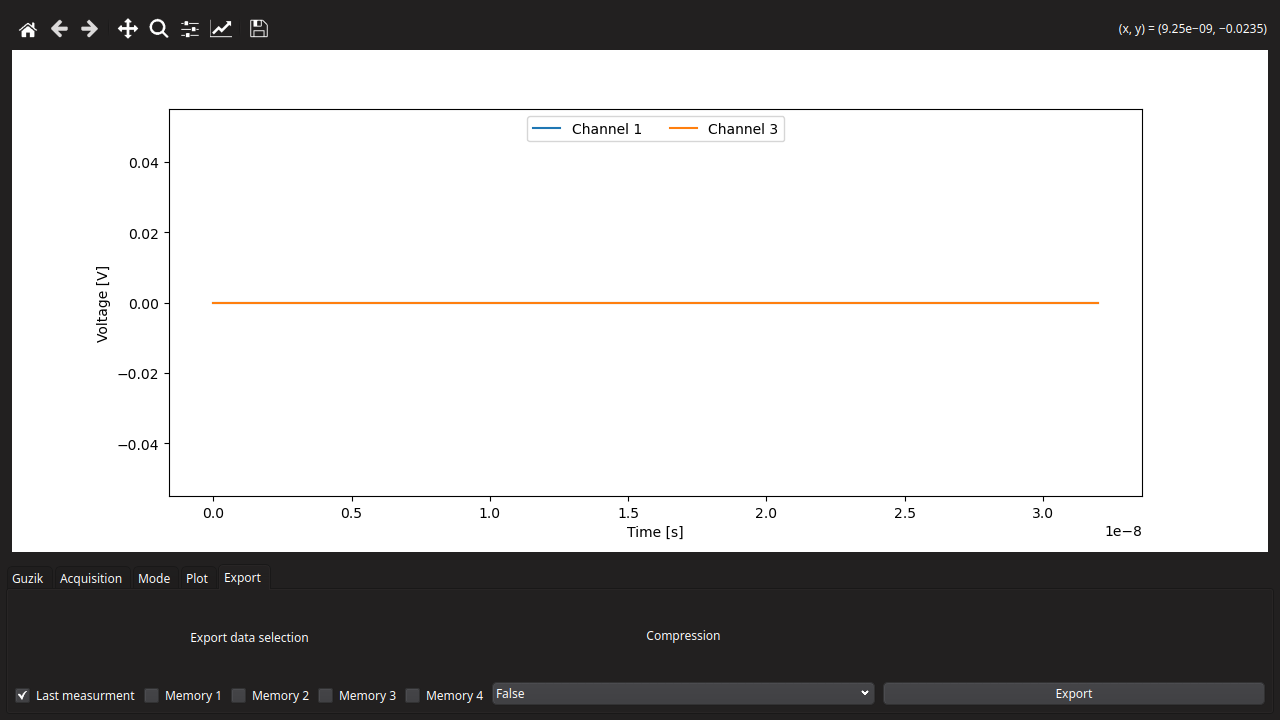
\includegraphics[width=\textwidth]{Figures/Export.png}
\end{center}
\clearpage\null\thispagestyle{empty}

\end{document}
